\documentclass[11pt,landscape,a4paper]{article}
\usepackage[utf8]{inputenc}
\usepackage[ngerman]{babel}
\usepackage[T1]{fontenc}
%\usepackage[LY1,T1]{fontenc}
%\usepackage{frutigernext}
%\usepackage[lf,minionint]{MinionPro}
\usepackage{tikz}
\usetikzlibrary{shapes,positioning,arrows,fit,calc,graphs,graphs.standard}
\usepackage[nosf]{kpfonts}
\usepackage[t1]{sourcesanspro}
\usepackage{multicol}
\usepackage{wrapfig}
\usepackage[top=2mm,bottom=2mm,left=2mm,right=2mm]{geometry}
\usepackage[framemethod=tikz]{mdframed}
\usepackage{microtype}
\usepackage{pdfpages}
\usepackage[shortlabels]{enumitem}

\newif\iflong
\longtrue % \longfalse for short version and \longtrue for long version
\newcommand{\inLongVersion}[1]{\iflong #1\fi}


\setlist{nosep}
\setlist[itemize]{leftmargin=*}
\setlist[enumerate]{leftmargin=*}

\newcommand{\score}{\text{score}}
\newcommand{\encoder}{\text{encoder}}
\newcommand{\decoder}{\text{decoder}}
\newcommand{\E}{\mathbb{E}}
\newcommand{\Dist}{\mathcal{D}}
\newcommand{\normal}{\mathcal{N}}
\DeclareMathOperator{\cov}{\textbf{Cov}}
\DeclareMathOperator{\var}{\textbf{Var}}
\DeclareMathOperator{\argmin}{\textbf{argmin}}
\DeclareMathOperator{\argmax}{\textbf{argmax}}
\DeclareMathOperator{\sgn}{\textbf{sgn}}
\DeclareMathOperator{\dir}{\textbf{Dir}}
\DeclareMathOperator{\cat}{\textbf{Cat}}






\let\bar\overline

\definecolor{myblue}{cmyk}{0,0,0,1}


\def\firstcircle{(0,0) circle (1.5cm)}
\def\secondcircle{(0:2cm) circle (1.5cm)}

\colorlet{circle edge}{myblue}
\colorlet{circle area}{myblue!5}

\tikzset{filled/.style={fill=circle area, draw=circle edge, thick},
    outline/.style={draw=circle edge, thick}}
    
\pgfdeclarelayer{background}
\pgfsetlayers{background,main}

\everymath\expandafter{\the\everymath \color{myblue}}
\everydisplay\expandafter{\the\everydisplay \color{myblue}}

\renewcommand{\baselinestretch}{.8}
\pagestyle{empty}

\global\mdfdefinestyle{header}{%
linecolor=gray,linewidth=1pt,%
leftmargin=0mm,rightmargin=0mm,skipbelow=0mm,skipabove=0mm,
}

\newcommand{\header}{
\begin{mdframed}[style=header]
\footnotesize
\sffamily
\centering
AML, Yuhao Mao,~Page~\thepage
\end{mdframed}
}

\makeatletter % Author: https://tex.stackexchange.com/questions/218587/how-to-set-one-header-for-each-page-using-multicols
\renewcommand{\section}{\@startsection{section}{1}{0mm}%
                                {.5ex}%
                                {.5ex}%x
                                {\color{myblue}\sffamily\bfseries}}
\renewcommand{\subsection}{\@startsection{subsection}{2}{0mm}%
                                {.2ex}%
                                {.2ex}%x
                                {\sffamily\bfseries}}
\renewcommand{\subsubsection}{\@startsection{subsubsection}{3}{0mm}%
                                {.1ex}%
                                {.1ex}%x
                                {\sffamily\itshape}}



\def\multi@column@out{%
   \ifnum\outputpenalty <-\@M
   \speci@ls \else
   \ifvoid\colbreak@box\else
     \mult@info\@ne{Re-adding forced
               break(s) for splitting}%
     \setbox\@cclv\vbox{%
        \unvbox\colbreak@box
        \penalty-\@Mv\unvbox\@cclv}%
   \fi
   \splittopskip\topskip
   \splitmaxdepth\maxdepth
   \dimen@\@colroom
   \divide\skip\footins\col@number
   \ifvoid\footins \else
      \leave@mult@footins
   \fi
   \let\ifshr@kingsaved\ifshr@king
   \ifvbox \@kludgeins
     \advance \dimen@ -\ht\@kludgeins
     \ifdim \wd\@kludgeins>\z@
        \shr@nkingtrue
     \fi
   \fi
   \process@cols\mult@gfirstbox{%
%%%%% START CHANGE
\ifnum\count@=\numexpr\mult@rightbox+2\relax
          \setbox\count@\vsplit\@cclv to \dimexpr \dimen@-1cm\relax
\setbox\count@\vbox to \dimen@{\vbox to 1cm{\header}\unvbox\count@\vss}%
\else
      \setbox\count@\vsplit\@cclv to \dimen@
\fi
%%%%% END CHANGE
            \set@keptmarks
            \setbox\count@
                 \vbox to\dimen@
                  {\unvbox\count@
                   \remove@discardable@items
                   \ifshr@nking\vfill\fi}%
           }%
   \setbox\mult@rightbox
       \vsplit\@cclv to\dimen@
   \set@keptmarks
   \setbox\mult@rightbox\vbox to\dimen@
          {\unvbox\mult@rightbox
           \remove@discardable@items
           \ifshr@nking\vfill\fi}%
   \let\ifshr@king\ifshr@kingsaved
   \ifvoid\@cclv \else
       \unvbox\@cclv
       \ifnum\outputpenalty=\@M
       \else
          \penalty\outputpenalty
       \fi
       \ifvoid\footins\else
         \PackageWarning{multicol}%
          {I moved some lines to
           the next page.\MessageBreak
           Footnotes on page
           \thepage\space might be wrong}%
       \fi
       \ifnum \c@tracingmulticols>\thr@@
                    \hrule\allowbreak \fi
   \fi
   \ifx\@empty\kept@firstmark
      \let\firstmark\kept@topmark
      \let\botmark\kept@topmark
   \else
      \let\firstmark\kept@firstmark
      \let\botmark\kept@botmark
   \fi
   \let\topmark\kept@topmark
   \mult@info\tw@
        {Use kept top mark:\MessageBreak
          \meaning\kept@topmark
         \MessageBreak
         Use kept first mark:\MessageBreak
          \meaning\kept@firstmark
        \MessageBreak
         Use kept bot mark:\MessageBreak
          \meaning\kept@botmark
        \MessageBreak
         Produce first mark:\MessageBreak
          \meaning\firstmark
        \MessageBreak
        Produce bot mark:\MessageBreak
          \meaning\botmark
         \@gobbletwo}%
   \setbox\@cclv\vbox{\unvbox\partial@page
                      \page@sofar}%
   \@makecol\@outputpage
     \global\let\kept@topmark\botmark
     \global\let\kept@firstmark\@empty
     \global\let\kept@botmark\@empty
     \mult@info\tw@
        {(Re)Init top mark:\MessageBreak
         \meaning\kept@topmark
         \@gobbletwo}%
   \global\@colroom\@colht
   \global \@mparbottom \z@
   \process@deferreds
   \@whilesw\if@fcolmade\fi{\@outputpage
      \global\@colroom\@colht
      \process@deferreds}%
   \mult@info\@ne
     {Colroom:\MessageBreak
      \the\@colht\space
              after float space removed
              = \the\@colroom \@gobble}%
    \set@mult@vsize \global
  \fi}

\makeatother
\setlength{\parindent}{0pt}




\begin{document}
%\footnotesize
\small
\begin{multicols*}{4}

% input your sections here
\section{Adversarial Attacks}

\begin{itemize}
    \item Targeted FGSM: $x^\prime = x - \epsilon \sgn(\nabla_x \mathcal{L}_t(x))$, where $t$ is the target label. Untargeted FGSM: $x^\prime = x + \epsilon \sgn(\nabla_x \mathcal{L}_y (x))$, where $y$ is the original label.
    \item CW: use L-BFGS to solve $\argmin_\eta ||\eta||_p+c\cdot \text{obj}_t(x+\eta)$, s.t. $x+\eta\in [0,1]^n$.
\end{itemize}

\section{Certification of NN}

Goal: given a neural network $N$, a constraint over input $\phi$ and a property over outputs $psi$, prove that $\forall i \in I . i \vDash \phi \Rightarrow N(i) \vDash \psi$ or return a violation. We want sound, complete and efficient (scalable to large NN) algorithms, i.e., to either scale sound and complete methods or to make sound but incomplete methods more precise.

\subsection*{Sound vs Complete}
\begin{itemize}
    \item Sound: if the property is violated, the program always states the property is violated.
    \item Complete: if the property holds, the program always states the property holds.
\end{itemize}

Incomplete but sound methods include convex relaxations. Complete and sound methods include Mixed-Integer Linear Programming (MILP).

\subsection*{Convex Relaxations}
\begin{itemize}
    \item Box. Use intervals as the approximation.
    \item Zonotope. Represent every variable by $x_i = a^i_0+\sum_j a_j^i \epsilon_j = a_i^T e$, where $\epsilon_i\in [-1,1]$, $a_i\ge 0$. (1) The encoding for affine layer $y=Wx+b$ is $y=W A e+b$, which is exact. (2) To compute the encoding for ReLU layers, we first obtain box bounds by plugging in $\epsilon=-1$ and $\epsilon=1$. When it is strictly positive (negative), then use $y=x$ ($y=0$). For cross-boundary cases, use the line between $(l,0)$ and $(u,u)$ as the upper bound ($y=\lambda(x-l)$, $\lambda=\frac{u}{u-l}$) and its parallel as the lower bound ($y=\lambda x$). Then we compute the standard form of this zonotope by $y = \lambda(x-tl)$, $t\in [0,1]$, plug in $t=(\epsilon_{\text{new}}+1)/2$, $\epsilon_{\text{new}}\in [-1,1]$ and expand.
    \item DeepPoly. Represent every variable by $x_i \ge \sum_j w^l_j x_j + v^l$, $x_i \le \sum_j w^u_j x_j +v_j$ and $l_i \le x_i \le u_i$. First do a forward propagation and then a backward propagation. (1) For affine layer $y=Wx+b$, use $Wx+b\le y\le Wx+b$. (2) For ReLU layers, if it is strictly positive (negative), use $x\le y\le x$ ($0\le y\le 0$). Otherwise, apply min-area heuristic to choose one from $0\le y\le \lambda(x-l)$ and $\lambda x\le y \le \lambda(x-l)$, i.e., choose the first one if $|l|\ge|u|$ o.w. the second one. When forward-propagating, we compute the interval bound by back-substituting to the first layer.
\end{itemize}

Comparison between relaxations: as long as the relaxation of one method is not included by another, they cannot be compared, although one might have a smaller area.

\subsection*{Complete Methods}
\begin{itemize}
    \item MILP: complete for ReLU network at the cost that it is at least NP-complete. The standard form is to $\min c^T x$, s.t. $Ax \le_p b$, $l \le_p x[\mathcal{R}] \le_p u$ and $x[\neg\mathcal{R}] \in Z^k$, where $x[\mathcal{R}]$ means the continuous component of $x$ and $\le_p$ means point-wise comparison. (1) The encoding for affine layer is: $Wx+b\le y\le Wx+b$. (2) The encoding for ReLU is: $y\le x-l(1-a)$, $y\ge x$, $y\le u\cdot a$, $y\ge 0$ and $a\in\{0,1\}$. $a$ serves as a ``state'' indicator to encode a piece-wise linear function. (3) Assume the goal is to prove $o_0>o_1$, then we do $\min o_0-o_1$ and see if the outcome is positive. (4) $l,u$ are pre-computed by Box. MILP benefits from Box bounds in that it could stop further exploration of infeasible combinations of integer variables, e.g., if the objective lower bound is positive when $a_1=0$, then there is no need to explore $a_2$ for $a_1=0$.
\end{itemize}



\section{Certified Training}

Goal: train NN so that it has maximum certified accuracy.

\textbf{DiffAI} Formalization: 
$$\min_\theta \E_{x,y} \max_{x^\prime\in \gamma(NN^{\#}(S(x)))} \mathcal{L}(x^\prime, y;\theta)$$
where $S(x)$ is the allowed input set, $NN^{\#}$ is the abstraction of NN (e.g., DeepPoly abstraction). 
\begin{itemize}
    \item Suppose we use $\mathcal{L}(z, y) = \max_{q\ne y}(z_q-z_y)$. Then for each iteration, we first compute the convex relaxation of the input, and then compute the interval bound for $z_q-z_y$. Then we use the upper bound as the loss and update according to the gradient (Note that it is still differentiable).
    \item Suppose we use the cross entropy loss. Then we first compute the interval bound for $z_i$ and pick the upper bound for incorrect classes and lower bound for correct classes to form a new vector. Then we use this new vector to compute the cross entropy and update.
\end{itemize}
There are a few practical tricks:
\begin{enumerate}
    \item Start with a small $S(x)$ and then grow it.
    \item Dynamically switch between standard loss and the certified loss.
\end{enumerate}

To avoid increasing difficulty in the optimization due to better relaxations, Convex Layerwise Adversarial Training (\textbf{COLT}) is developed. The goal of COLT is to find a feasible point in the first-layer relaxation so that the loss is maximized and use this feasible point in the certified loss. When combined with Zonotope, it uses projection in the $\epsilon$ space since each $\epsilon \in [0,1]^n$ corresponds to a point in the zonotope. Although it is not the min-distance projection in the zonotope, it avoids the problem when the zonotope lies in a lower dimension where direct projection is not possible. It allows better results when a better relaxation is used.

\section{Logic in DL}

Goal: do query involving NN; forcing properties into NN.

\subsection*{NN Querying by Optimization}

Idea: translate properties $\phi$ into loss function $T$ and optimize it. 

Challenge: how to find a loss function such that $\forall x, T(\phi)(x)=0\Leftrightarrow x$ satisfies $\phi$. For example, $\phi$ could be: $|z-x|_{\infty}<\epsilon \Rightarrow |NN(z)-NN(x)|_{\infty}<\delta$. 

Useful rules:
\begin{itemize}
    \item $x\Rightarrow y$ is equivalent to $\neg x \lor y$.
    \item $\neg (x \lor y)$ is equivalent to $\neg x \land \neg y$.
    \item $\neg (x \land y)$ is equivalent to $\neg x \lor \neg y$. 
\end{itemize}


One possible translation (DL2) is:
\begin{enumerate}
    \item $t_1\le t_2 \longrightarrow \max(0, t_1-t_2)$.
    \item $t_1\ne t_2 \longrightarrow I(t_1=t_2)$.
    \item $t_1=t_2 \longrightarrow T(t_1\le t_2) + T(t_2\le t_1) = |t_1-t_2|$.
    \item $t_1<t_2 \longrightarrow T(t_1\le t_2) + T(t_1\ne t_2)$.
    \item $\phi \lor \psi \longrightarrow T(\phi)\cdot T(\psi)$.
    \item $\phi \land \psi \longrightarrow T(\phi) + T(\psi)$.
\end{enumerate}

Trick for box constraints: when the input is constrained by a box, pass it to the optimizer such as L-BFGS-B.

\subsection*{Forcing properties of NN}

Goal: $\max_\theta \E_{s\sim D}I(\forall z, \phi(z, s;\theta))$. Equivalently, $\min_\theta \E_{s\sim D} T(\phi)(z^*, s; \theta)$, where $z^* = \argmin_z T(\neg \phi)(z,s;\theta)$. Remember to take out any box constraints.

\section{Randomized Smoothing}

Given a base classifier $f$ (the NN), the smoothed classifier is defined as $g(x)=\argmax_c P(f(x+\epsilon)=c)$, where $\epsilon \sim \normal(0,\sigma^2 I)$.

Theorem: suppose $\exists \underline{p_A}, \bar{p_B} \in [0,1]$, s.t. $P(f(x+\epsilon)=c_A) \ge \underline{p_A} \ge \bar{p_B} \ge \max_{c\ne c_A} P(f(x+\epsilon)=c)$, then $g(x+\delta)=c_A$ for all $|\delta|_2 <R$, where $R=\frac{\sigma}{2} (\Phi^{-1}(\underline{p_A})-\phi^{-1}(\bar{p_B}))$, $\Phi^{-1}$ is the inverse of standard Gaussian CDF.

If we further require $\underline{p_A}>\frac{1}{2}$, then $\bar{p_B})<1-\underline{p_A}$ and thus $R>\sigma \Phi^{-1}(\underline{p_A})$. To compute probability, we use sampling. To avoid selection bias, we first sample to get the top label and then use an independent sampling to estimate the probability. The procedure is as follows:

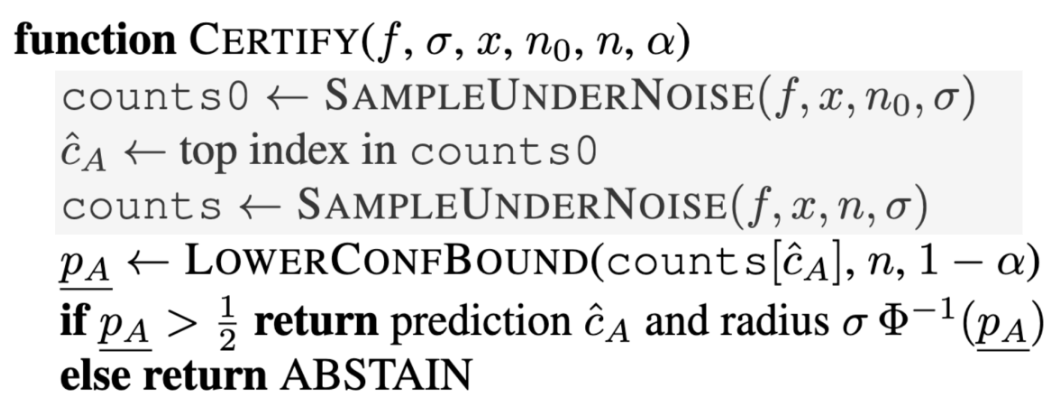
\includegraphics[width=\columnwidth]{img/rand_smooth.png}

At inference time, to compute $g(x)$, we need another sampling procedure:

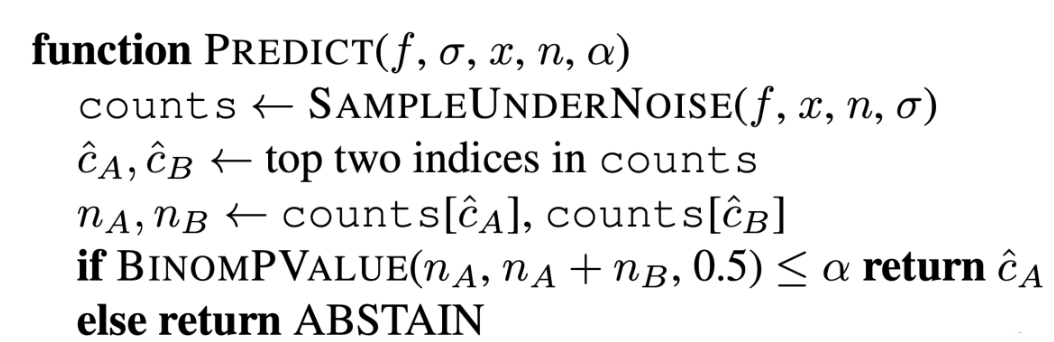
\includegraphics[width=\columnwidth]{img/rand-predict.png}

The probability of wrong prediction is $P(\hat{c_A}\ne c_A, \text{no abstain}) = P(\hat{c_A}\ne c_A)P(\text{no abstain} \mid \hat{c_A}\ne c_A) \le \alpha$.

Pros: (1) it can scale to large networks and (2) is model-agnostic.

Cons: (1) it requires sampling at inference time and (2) many samples could be needed to increase the certified radius.

\section{Certifying Geometric Transformations}

\begin{itemize}
    \item Rotation: $T_\phi(x, y) = (x\cos(\phi)-y\sin(\phi), x\sin(\phi)+y\cos(\phi))$.
    \item Translation: $T_{\delta_x, \delta_y}(x,y) = (x+\delta_x, y+\delta_y)$.
    \item Scaling: $T_\lambda(x,y) = (\lambda x,\lambda y)$.
    \item Bilinear interpolation for non-integer $(x,y)$: $I(x, y)=p_{x_{1}, y_{1}}\left(x_{2}-x\right)\left(y_{2}-y\right)+p_{x_{1}, y_{2}}\left(x_{2}-x\right)\left(y-y_{1}\right)+p_{x_{2}, y_{1}}\left(x-x_{1}\right)\left(y_{2}-y\right)+p_{x_{2}, y_{2}}\left(x-x_{1}\right)\left(y-y_{1}\right)$, where $x_1\le x\le x_2$, $y_1\le y\le y_2$, $x_2=x_1+1$ and $y_2=y_1+1$.
\end{itemize}

\subsection*{DeepG}

Idea: use convex approximation for the exact input set. DeepG use the shape of DeepPoly but use a different strategy. It bounds all operations done in the $I_\kappa$ simultaneously, and thus is more tight than DeepPoly.

DeepG finds two planes such that $w_l^T \kappa+b_l \le I_\kappa \le w_u^T\kappa+b_u$, where $\kappa$ is the hyperparameter of transformation. It uses the min-volume heuristic: $w_l, b_l = \argmin \E (I_\kappa - (w_l^T \kappa+b_l))$. Using linear programming, we can solve this optimization for a finite number of sampled points.

To extend the soundness to the whole hyperparameter space, we can modify the constraint by translating the plane, i.e., use $b_l = \hat{b_l}-\delta_l$ and $b_u = \hat{b_u}+\delta_u$. We can compute $\delta$ by either using box relaxation on $f(\kappa)=\hat{w_l}^T\kappa+\hat{b_l}-I_\kappa$, or by using Lipschitz and mean-value theorem on $f(\kappa)$: $f(\kappa)-f(\frac{1}{2}(h_u+h_l))\le |L|^T(\frac{1}{2}(h_u-h_l))$, where $\kappa \in [h_l, h_u]$. After deriving the convex relaxation for the transformation, we can use DeepPoly to complete the verification. To further improve the approximation, we can decompose the hyperparameter space, and validate each of them separately.

\section{Fairness}

\subsection*{Individual Fairness}

Goal: for similar inputs, give similar outputs. 

Key: define similarity $\phi(x,x^\prime)\rightarrow \{0,1\}$. Then use DL2 to translate the similarity constraint into loss functions.

\begin{itemize}
    \item Pre-process (data producer): provably learn a representation $z=f_\theta$ s.t. $\phi(x,x^\prime)\Rightarrow |z-z^\prime|_2<\delta$.
    \item In-process (data consumer): provably learn a classifier $h_\psi$ s.t. $|z-z^\prime|_2<\delta \Rightarrow h_\psi(z) = h_\psi(z^\prime)$.
\end{itemize}

\subsection*{Group Fairness}

Goal: $P(Y\mid G=0)=P(Y\mid G=1)$, e.g., fairness w.r.t. race and gender.

\begin{itemize}
    \item Ignore target features. Usually does not work due to the correlation between features.
    \item Estimate probability and use PAC framework.
\end{itemize}

\section{Federated Learning}

Types of Federated Learning:
\begin{enumerate}
    \item Cross-device. (1) Huge \#sources, (2) each with small amount of data, (3) dynamically drop in and out in the learning process, (4) contact rarely. Example: Google spell checker.
    \item Cross-sillo. (1) Limited \#sources, (2) each with a lot of data, (3) participate constantly, (4) potentially heterogeneous. Example: Hospitals MRI segmentation.
\end{enumerate}

Learning Epoch: (1) server selects clients to participate; (2) local computation on private data and send information to the server; (3) aggregation of local information on the server; (4) send aggregated information to clients.

\subsection*{Common Algorithms}
\begin{itemize}
    \item FedSGD. Do one iteration of local SGD on global weights and average them as the global update. Pros: It has convergence guarantee. Cons: Expensive communication.
    \item FedAvg. Do several iterations of local SGD on the global weights and average the local weights as the global weight. Pros: Less communication. Cons: No guarantee of convergence.
\end{itemize}

\subsection*{Common Issues}
\begin{itemize}
    \item Honest-but-Curious Server: honestly follow the algorithm but want to expose private data of clients. Gradient inversion: match gradients of reconstructed and client data.
    \item Client-side poisoning: send crafted updates to the server to force divergence or bad behavior on certain data. 
    \item Client fairness: model behaves well on average but poorly for certain clients due to heterogeneity. There is a trade-off between preventing client-side poisoning and client fairness because the server cannot tell whether a bad update is malicious or because of heterogeneity.
\end{itemize}

\subsection*{Defenses}

Differential Privacy. Definition: a randomized algorithm $M$ is differentially private w.r.t. $\epsilon$ and $\delta$ iff for all similar dataset $D, D^\prime$ ($|D-D^\prime|=1$) and all subsets of outputs, $P(M(D)\in S) \le e^\epsilon P(M(D^\prime)\in S)+\delta$.

\begin{itemize}
    \item Clip the gradient and add noises to it to achieve DP.
    \item Customization of the local model. Allowing clients to use the global model and customize locally can help to solve the dilemma.
\end{itemize}

\section{Abstract Interpretation}
Theory of approximation.

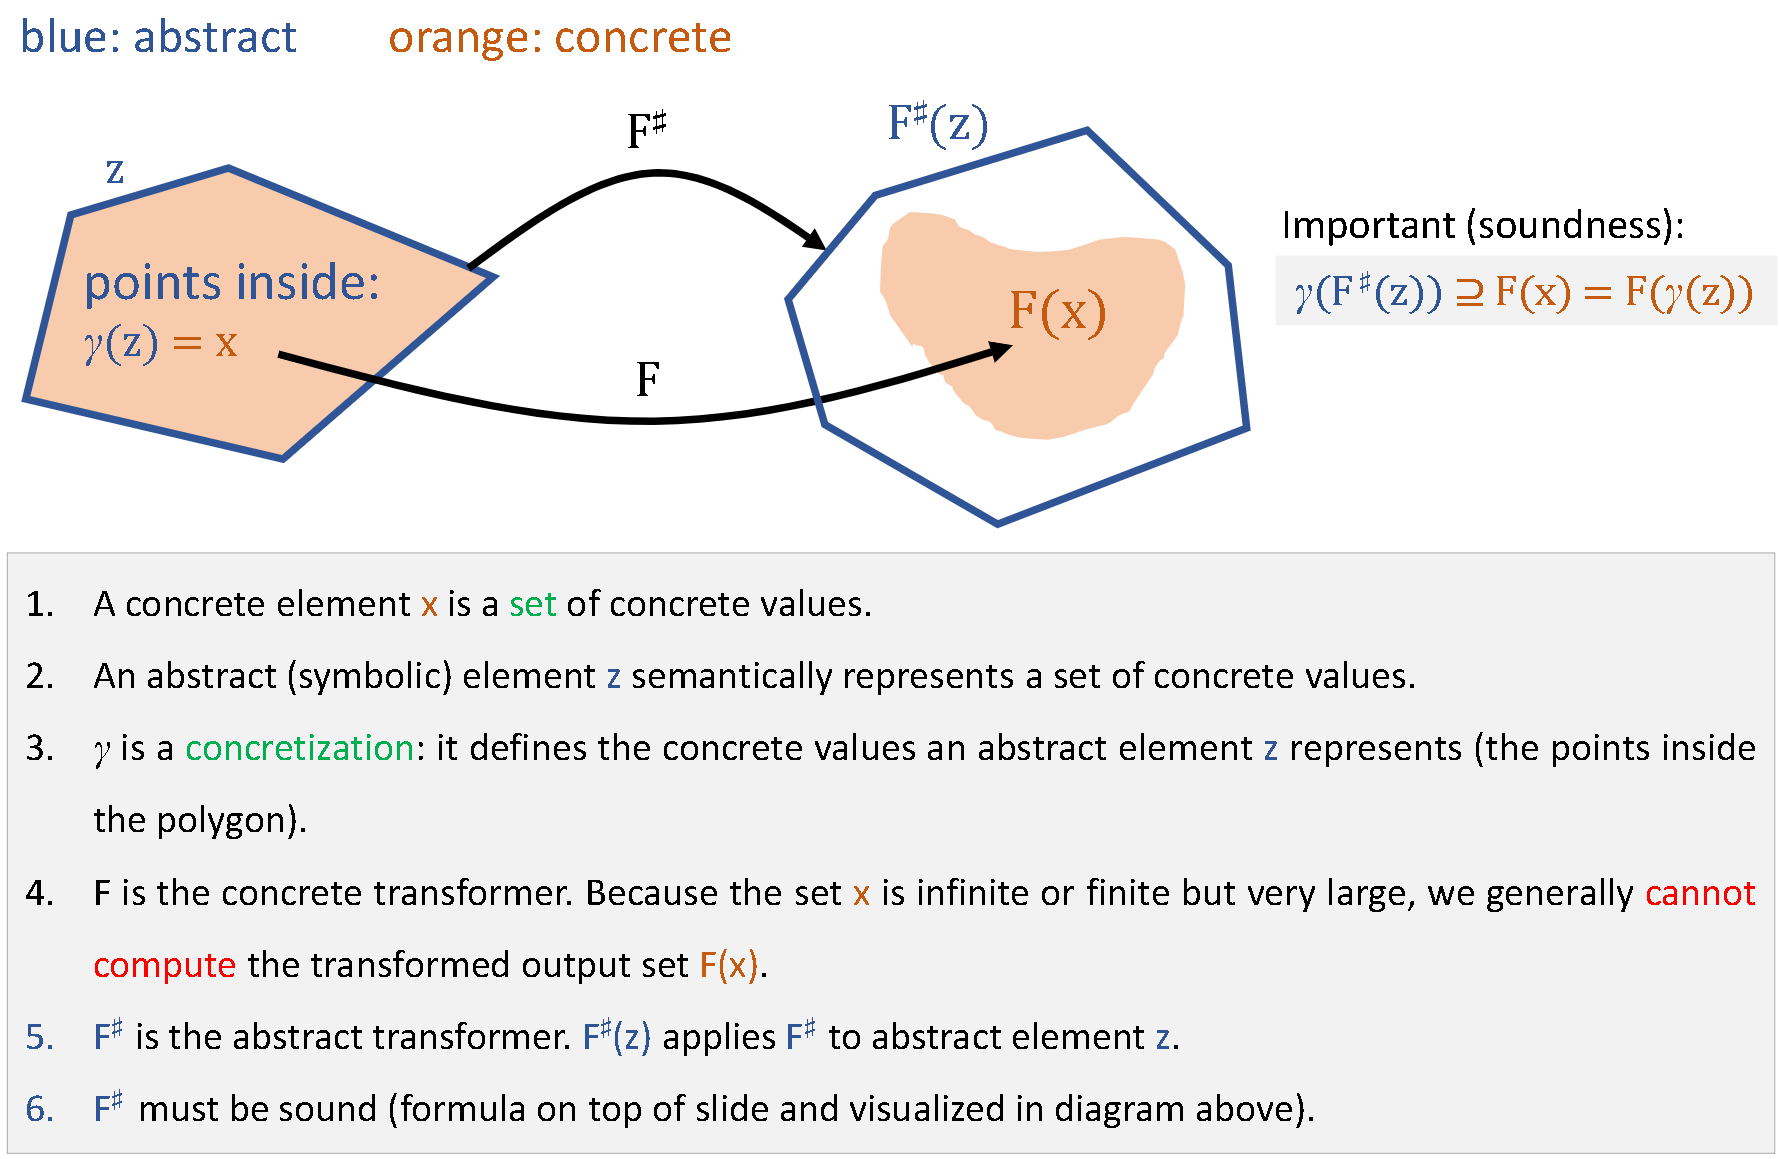
\includegraphics[width=2\columnwidth]{img/abstract_interpret.png}

\end{multicols*}
\end{document}